\documentclass{article}[12pt]

\usepackage[francais]{babel}
\usepackage{boxedminipage}
\usepackage[utf8]{inputenc}
\usepackage{amsfonts,amssymb,amsmath}
\usepackage{graphicx}
\usepackage{vmargin}
\usepackage{grffile} 
\setpapersize{A4}
\setmarginsrb{2cm}{2cm}{2cm}{2cm}{0cm}{0cm}{0cm}{0cm} 

\setlength{\parindent}{0pt}

%\setlength{\textwidth}{17cm}
%\setlength{\evensidemargin}{0pt}
%\setlength{\oddsidemargin}{0pt}
%\setlength{\topmargin}{0pt}


\begin{document}
\begin{center}
\framebox[1.07\width]{
\begin{minipage}[b]{4cm}
%\includegraphics[width=4.5cm]{LOGO_EM.pdf}  
\end{minipage} 
\begin{minipage}[b]{11cm}
\ \\[.1cm]
%%%%%%%%%%%%%%%%%%%
%   ANNÉE 
Année 2021-2022
%%%%%%%%%%%%%%%%%%%
\hspace{\stretch{1}} 
%%%%%%%%%%%%%%%%%%%
% NUMERO DE SESSION
$1^\textrm{ère}$ session 
%%%%%%%%%%%%%%%%%%%
\\[.15cm]
\begin{center}
%%%%%%%%%%%%%%%%%%%
% DONNÉES DU MODULE
\textsc{Algorithmique Distribu\'ee}\\
\textsc{IF223}\\
\textsc{Rohan Foss\'e}\\
%%%%%%%%%%%%%%%%%%%
\end{center}
\ \\[.2cm]
%%%%%%%%%%%%%%%%%%%
% Données diverses
Filière : {T\'el\'ecom}
\hspace{\stretch{1}}
Année : {2022}
\hspace{\stretch{1}}
Semestre : {2}
\\[.2cm]
Date de l'examen : {23 Mai 2022}
\hspace{\stretch{1}}
Durée de l'examen : {1h}
%%%%%%%%%%%%%%%%%%%
\\[.2cm]
\begin{tabular}{llll}
%%%%%%%%%%%%%%%%%%%
% remplacer $\Box$ par $\boxtimes$ pour cocher.
Documents autorisés &  $\boxtimes$     & %\hspace{.5cm} &
sans document & $\Box$ \\
Calculatrice autorisée & $\boxtimes$ &
non autorisée & $\Box$ \\
% remplacer $\Box$ par $\boxtimes$ pour cocher.
\end{tabular}
\\[.2cm]
%Autre : {.......}
\\[.2cm]
\end{minipage}
}

\end{center}

\vspace{1cm}
\begin{center}\huge{\textbf{SUJET}}\end{center}
\vspace{1cm}

%%%%%%%%%%%%%%%%%%%
% DÉBUT DU SUJET
%%%%%%%%%%%%%%%%%%%

\begin{center}
  \begin{boxedminipage}{\linewidth}
    {\large {\bf Nom et Prénom} :}~\\
  \end{boxedminipage}
\end{center}

\textbf{
\begin{itemize}
\item Toutes les parties du sujet sont indépendantes (en particulier les exercices) ;
\item Il est impératif de répondre dans les espaces prévus à cet effet : ce qui dépasse
  ne sera pas lu. Pour les parties où il faut écrire du code, merci d'écrire une ligne
  devant chaque numéro. \textbf{Vous êtes donc limités dans la quantité de code que vous êtes
  autorisés à écrire pour chaque question.}
\item Merci d'écrire dans un français correct : orthographe, grammaire et conjugaison
  seront pris en compte dans la correction ;
\item Vos codes doivent être indentés correctement ;
\item Merci de retirer les pages d'annexe du sujet avant de me rendre votre copie ;
\item Enfin, n'oubliez pas d'indiquer votre NOM sur la copie !
\end{itemize}
}

\section{Coloration des cycles}


Dans cette partie on considère exclusivement des algorithmes distribués s’exécutant dans le modèle
LOCAL. La couleur d’un sommet u sera toujours identifiée par une variable notée $Color(u) \in \mathcal{N}$.
Le sommet u, quant à lui, sera identifié par Id(u). Les graphes seront considérés comme non-orientés.
Pour un cycle cela signifie qu’il n’y a pas de notion de successeur et de prédécesseur coordonnée entre
les sommets. Il n’y a pas de variable Parent par exemple. Un sommet peut seulement envoyer ou
recevoir des messages d’un ou plusieurs de ses voisins sans pouvoir déterminer quel voisin est à sa
droite par exemple.\\


    \textbf{Question 1:} Rappeler les caractéristiques du modèle LOCAL.\\
    
    \textbf{Question 2:} On suppose donnée une 6-coloration d'un cycle. Donner un algorithme produisant en une seule ronde une 4-coloration.\\
    
    \textbf{Question 3:} En déduire un algorithme en deux rondes permettant de passer de 6 à 3 couleurs dans un cycle.\\


On dira qu’un cycle possède une (a, b)-coloration si chaque sommet u possède une couleur $Color(u) \in \{1, 2\}$ de sorte qu’il y ait au plus a sommets de couleur 1 et b sommets de couleur 2 consécutifs sur le cycle. Ainsi une (1, 1)-coloration d’un cycle de longueur paire est simplement une
2-coloration classique (alternance des couleurs 1 et 2). Notez que contrairement à une k-coloration
classique, une (a, b)-coloration peut avoir deux voisins d’une même couleur dès que a $>$ 1 ou b $>$ 1.\\

\textbf{Question 4:} Montrer qu’une (1, 2)-coloration définit un ensemble indépendant maximal, c’est-à-dire un sous-ensemble de sommets deux à deux non-adjacents et qui soit maximal pour l’inclusion.\\

\textbf{Question 5:} Donner un algorithme permettant de produire une 3-coloration pour un cycle à partir
d’une (1, 2)-coloration. Préciser le nombre de rondes qui devra être aussi faible que possible.\\

\textbf{Question 6:} Généraliser votre algorithme de façon à produire une 3-coloration à partir d’une (a, b)-coloration, tout en précisant le nombre de rondes. Vous pourrez supposer que les valeurs a et b sont connues de tous les sommets.\\


\section{Election dans un arbre}

Nous allons considérer un algorithme d’élection sur l’arbre. Il est décomposé en deux phases.
La première phase est une phase de réveil. La seconde phase correspond à la phase de calcul de
leader des feuilles à la racine tel que un site donne le résultat à son père lors qu’il connaît la
valeur maximun de son sous-arbre. Voici la description plus précise de cet algorithme :

\begin{enumerate}
    \item Réveiller tous les sommets à partir d’un seul un initiateur. Le sommet initiateur sera la
racine.

\item Calculer la plus grande étiquette de l’arbre (le gagnant étant le sommet qui possède cette
étiquette). Pour cela:

\begin{enumerate}
    \item Faire un parcours des feuilles vers l’intérieur de l’arbre en calculant la plus petite
étiquette au fur et à mesure.
\item Propager le résultat de l’élection de voisin en voisin. Si un sommet reçoit son étiquette,
il se déclare vainqueur, sinon perdant.


\end{enumerate}
\end{enumerate}

\textbf{Question 1:}
Écrire de façon formelle cet algorithme\\

\textbf{Question 2:} Proposer une exécution possible sur l'arbre de la figure 1\\

\begin{figure}[h!]
    \centering
    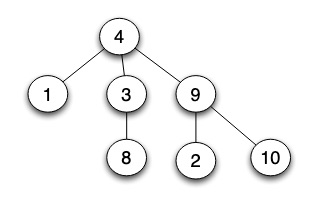
\includegraphics[scale=0.8]{a3.jpg}
    \caption{Arbre de 8 sommets}
    \label{fig:my_label}
\end{figure}

\textbf{Question 3:} Ecrire un algorithme réparti qui vérifie si le réseau est un arbre
\end{document}
